\newpage
%%\chapter{Diagramas}
%%\label{chap:diagrams}
 

\chapter{Manual de uso}
\label{chap:usage}

\lettrine{E}{n} este apéndice se detallan aspectos de los módulos que no se encuentran en la propia documentación en Javadoc del código, y que son necesarios para el buen funcionamiento de los mismos.

\section{Carga de módulos}

A la hora de cargar los módulos necesarios para la aplicación, se necesita declararlos en un fichero \textit{modules.properties} que debe colocarse en la carpeta \textbf{assets} de la aplicación. Los módulos son declarados de la forma que se indica en la figura \ref{fig:module-declaration}, escribiendo el espacio de nombres hasta llegar a la implementación específica del módulo que se desee emplear.
El orden de la declaración de módulos es importante, ya que es el que se seguirá a la hora de cargarlos al ejecutar la aplicación se deben tener en cuenta las dependencias entre módulos, por ejemplo, no declarando el \textit{FaceDetectionModule} antes que el \textit{BasicCameraModule}.
\begin{figure}
	\centering
	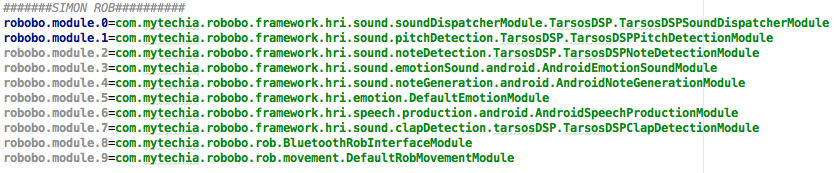
\includegraphics[width=1.1\linewidth]{imagenes/moduledeclaration.png}
	\caption{Declaración de los módulos para el ejemplo del Simon dice musical}
	\label{fig:module-declaration}
\end{figure}

Para usar los módulos declarados en el fichero de propiedades es necesario utilizar la clase \textit{RoboboManager} que proporciona el método \textit{getModuleInstance}. En la figura \ref{fig:module-instantiation} se puede ver el proceso de instanciación e inicialización para los módulos del ejemplo del Simón dice musical. En dicha figura \textit{robobo} es la instancia del \textit{RoboboManager}.

\begin{figure}
	\centering
	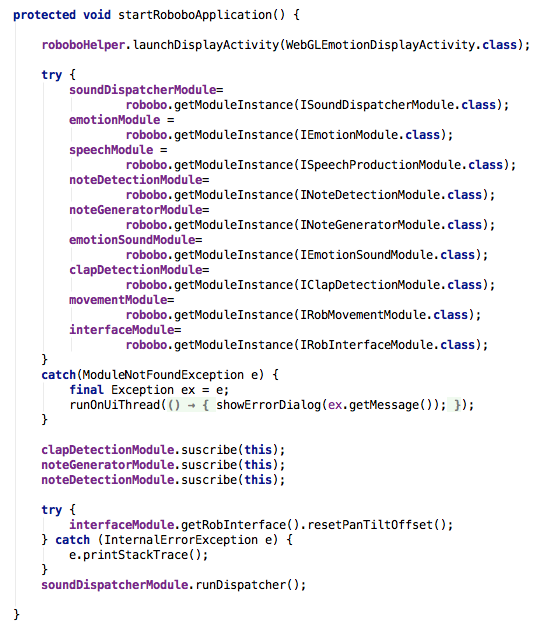
\includegraphics[width=1\linewidth]{imagenes/moduleinstantiation.png}
	\caption{Instanciación de los módulos para el ejemplo del Simon dice musical}
	\label{fig:module-instantiation}
\end{figure}


\section{Librería Speech}
\subsection{Módulo Production}
\label{manual:speechproduction}

El módulo SpeechProduction no requiere de ninguna consideración especial.

\subsection{Módulo Recognition}
\label{manual:speechrecognition}

Para el uso del modulo Recognition implementado con PocketSphinx es necesario tener en cuenta ciertos aspectos previos:

\begin{itemize}
	\item Debe crearse una carpeta \textbf{sync} en el directorio \textbf{assets} de la aplicación, en el interior de la cual se deben introducir tanto el modelo de lenguaje como el diccionario provistos con pocketsphinx.
	\item Dentro de la carpeta sync es necesario un archivo \textit{assets.lst}, en el cual deben declararse todos los archivos que se encuentren dentro del directorio \textbf{sync}.
	\item Todo archivo que se añada o modifique en la carpeta \textbf{sync} debe ir acompañado de un archivo que contenga su firma md5, por ejemplo, en el caso de de querer introducir una nueva gramática \textit{gramatica.gram}, deberá ser acompañado por el archivo \textit{gramatica.gram.md5}. Este fichero md5 no debe ser declarado en el fichero \textit{assets.lst} que se menciona en el punto anterior.
	\item El inicio del reconocedor de voz se realiza de manera asíncrona e interactuar con el antes de su completo arranque puede producir errores. Para evitar esta clase de fallos se notificará del arranque del mismo a través del evento \textit{onModuleStart()} declarado en el listener \textit{ISpeechRecognitionListener}.
	\item Para funcionar correctamente debe estar declarado el permiso \begin{verbatim} <uses-permission android:name="android.permission.RECORD_AUDIO" /> \end{verbatim} en el AndroidManifest.
		
	
\end{itemize}

La creación de gramáticas se hace a través del formato JSFG, a continuación se verá un ejemplo:

\begin{verbatim}
#JSGF V1.0;

grammar movements;

<starter> = rob;
<direction> =front|back|up|down|right|left;
<ending> = now;
public <movements> = <starter> <direction> <ending>;
\end{verbatim}

En este ejemplo se define una gramática para detectar comandos de movimiento estructurados. Solo se detectarán aquellas estructuras marcadas como public, como en este caso lo sería \textit{movements}, que esta formada por un símbolo de inicio\textit{starter}, una dirección \textit{direction} y un símbolo de finalización \textit{ending}, así, una frase valida en este sistema podría ser \enquote{rob front now}, mientras que \enquote{front now} o \enquote{rob front} serían ignoradas por el sistema.

Se pueden consultar los detalles de este tipo de gramáticas en la página del proyecto\cite{JSFGGrammar}.

\label{manual:speechrecognition}

\section{Librería Touch}
\subsection{Módulo Touch}
\label{manual:touchmodule}

El único detalle a tener en cuenta a la hora de utilizar el \textit{TouchModule} es la necesidad de pasarle los \textit{TouchEvent} capturados desde la actividad activa en ese momento, en la figura \ref{fig:feed-touchevent} puede verse el proceso.

\begin{figure}
	\centering
	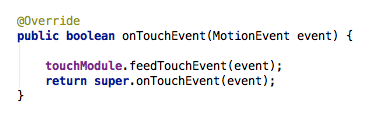
\includegraphics[width=0.7\linewidth]{imagenes/feedingtouchevent.png}
	\caption{Paso de los TouchEvents al módulo Touch}
	\label{fig:feed-touchevent}
\end{figure}

\section{Librería Vision}
\subsection{Módulo BasicCamera}
\label{manual:basiccamera}
El módulo BasicCamera necesita tener en cuenta varios aspectos para su correcto funcionamiento:
	\begin{itemize}
		\item Debe colocarse en la carpeta \textbf{assets} el archivo \textit{vision.properties}, donde se especificará la resolución de las imágenes capturadas de la siguiente manera:
		\begin{verbatim}
			resolution_height= 640
			resolution_width = 480
		\end{verbatim}
		\item Se necesita el permiso \begin{verbatim} <uses-permission android:name="android.permission.CAMERA" />\end{verbatim} para su correcto funcionamiento declarado en en \textit{AndroidManifest.xml}
	\end{itemize}
	
La tasa de captura de imágenes es de 2 frames por segundo en el smartphone empleado para el desarrollo y las pruebas, BQ Aquaris M5, pero se tiene constancia de que esta cifra varía al cambiar de terminal.
	
\subsection{Módulo FaceDetection}
\label{manual:facedetection}

El único aspecto a tener en cuenta en el módulo de reconocimiento facial es su dependencia hacia el \textit{BasicCameraModule}, que debe ser declarado antes que el de detección de caras en el \textit{modules.properties}

\subsection{Módulo ColorDetection}
\label{manual:colordetection}

Para el correcto funcionamiento del modulo detector de color es necesario tener en cuenta varios detalles:
\begin{itemize}
	\item Depende directamente del módulo \textit{BasicCameraModule}, que debe ser declarado antes que el de detección de colores en el fichero \textit{modules.properties}
	\item Depende de la librería OpenCV, por ello, el smartphone que vaya a utilizar este módulo necesitará tener instalada previamente la aplicación \textbf{OpenCVManager}.
	\item La resolución de las imágenes a procesar afecta directamente al rendimiento del módulo.
\end{itemize}

\section{Librería Sound}

\subsection{Módulo SoundDispatcher}
\label{manual:sounddispatcher}

El módulo \textit{SoundDispatcher} debe ser configurado en el archivo \textit{sound.properties} definiendo las siguientes características:
\begin{verbatim}
	samplerate = 44100
	buffersize = 2048
	overlap = 1024
\end{verbatim}

Dichas características se refieren a:

\begin{itemize}
	\item \textbf{Samplerate} hace referencia a la frecuencia de muestreo del sonido.
	\item \textbf{Buffersize} define el tamaño del buffer de audio.
	\item \textbf{Overlap} define el solapamiento entre muestras adyacentes.
\end{itemize}


Este módulo requiere el permiso \begin{verbatim} <uses-permission android:name="android.permission.RECORD_AUDIO" /> \end{verbatim} declarado en el AndroidManifest de la aplicación.

Para comenzar el procesado de audio debe llamarse al método del módulo \textit{runDispatcher()}, de lo contrario no funcionará ningún módulo que dependa de este.


\subsection{Módulo PitchDetection }
\label{manual:pitchdetection}

El modulo \textit{PitchDetection} depende directamente del módulo \textit{SoundDispatcher}, que debe ser declarado en el archivo \textit{modules.properties} antes que el \textit{PtichDetectionModule}.

\subsection{Módulo ClapDetection}
\label{manual:clapdetection}

Deben tenerse en cuenta varios detalles antes de poder utilizar el módulo \textit{ClapDetection}:
\begin{itemize}
	\item Depende directamente del módulo \textit{SoundDispatcher} que debe ser declarado previamente en el \textit{modules.properties} de la aplicación.
	\item Este módulo debe ser configurado en el archivo \textit{sound.properties}, definiendo las siguientes características, siendo ambas parametros de sensibilidad del detector de palmadas:
	\begin{verbatim}
		clap_threshold = 8
		clap_sensitivity = 50
	\end{verbatim}
\end{itemize}

\subsection{Módulo NoteDetection}
\label{manual:notedetection}

Deben tenerse en cuenta varios detalles antes de poder utilizar el módulo \textit{NoteDetection}:
\begin{itemize}
	\item Depende directamente del módulo \textit{PitchDetection}, y por tanto del \textit{SoundDispatcher} también, que deben ser declarados previamente en el \textit{modules.properties} de la aplicación.
	\item Este módulo debe ser configurado en el archivo \textit{sound.properties}, definiendo las siguientes características	\begin{verbatim}
		minThreshold = 0.1
		maxThreshold = 0.9
	\end{verbatim}
	Las dos características hacen referencia al porcentaje de desafinado permitido respecto al índice de una nota para considerarla válida.
\end{itemize}


\subsection{Módulo NoteGenerator}
\label{manual:notegenerator}

El módulo \textit{NoteGenerator} no requiere de indicaciones especiales.
\label{manual:emotionsound}
\subsection{Módulo EmotionSound}

El módulo \textit{EmotionSound} debe ser empleado con cautela, ya que si dos sonidos son reproducidos en un corto intervalo de tiempo podrían solaparse.


\section{Librería Messaging}
\subsection{Módulo Messaging}
\label{manual:messaging}
Varios aspectos deben tenerse en cuenta antes de usar el módulo de mensajería:
\begin{itemize}
	\item Debe configurarse la cuenta de correo que se vaya a utilizar para el envío de mensajes en el archivo \textit{messaging.properties}
	\begin{verbatim}
		emailaccount = xxxxxxxxxxxx@gmail.com
		emailpasswd = xxxxxxxx
	\end{verbatim}
	
	\item Deben añadirse los siguientes permisos al AndroidManifest de la aplicación:
	\begin{verbatim}
	<uses-permission android:name="android.permission.ACCESS_NETWORK_STATE" />
	<uses-permission android:name="android.permission.INTERNET" />
	<uses-permission android:name="android.permission.READ_EXTERNAL_STORAGE" />
	<uses-permission android:name="android.permission.WRITE_EXTERNAL_STORAGE" />
	\end{verbatim}
\end{itemize}
\newpage
\thispagestyle{empty}


















